% Compile from the repository root:
% latexmk -pdf -cd -interaction=nonstopmode -halt-on-error -outdir=../../tmp/pdfs \
%   output/pdf/ito_tracers_technical_note.tex
\documentclass[11pt]{article}

\usepackage[T1]{fontenc}
\usepackage{amsmath}
\usepackage{booktabs}
\usepackage{enumitem}
\usepackage{geometry}
\usepackage{graphicx}
\usepackage{hyperref}
\usepackage{microtype}
\usepackage{pdflscape}
\usepackage{tabularx}
\usepackage{xcolor}

\geometry{margin=0.85in}
\graphicspath{{../../docs/source/modules/figures/}}
\hypersetup{
  colorlinks=true,
  linkcolor=blue!55!black,
  urlcolor=blue!55!black,
  pdftitle={Second-Moment Ito Mass-Flux Tracers in AthenaK},
  pdfauthor={AthenaK feature ito tracers implementation note}
}
\setlist{nosep,leftmargin=1.5em}
\setlength{\parindent}{0pt}
\setlength{\parskip}{0.55em}
\newcommand{\Ito}{It\^o}
\newcommand{\AthenaK}{AthenaK}
\newcommand{\artifact}[1]{\path{#1}}
\newcommand{\status}[1]{\textbf{#1}}

\title{\textbf{Second-Moment \Ito{} Mass-Flux Tracers in \AthenaK{}}\\
\large Implementation Decisions, Validation, and Thermodynamic Tracing}
\author{Technical note for \texttt{feature/ito\_tracers}}
\date{Implementation baseline: commit \texttt{ab2c03880}, June 5, 2026}

\begin{document}
\maketitle

\begin{abstract}
The goal was to add the second-order \Ito{} tracer method to \AthenaK{} as a
continuous-path alternative to the existing Monte Carlo mass-flux tracers,
while explicitly excluding the third-order method. The implementation derives
cell-centered drift and diffusion coefficients from the same final
Runge--Kutta-weighted mass fluxes used by the Monte Carlo tracer, communicates
those coefficients across MeshBlocks and refinement boundaries, interpolates
them to each particle, and advances particles with an Euler--Maruyama step.

The evidence supports a precise conclusion: the implemented \Ito{}-2 particles
match the Monte Carlo tracer's per-coordinate displacement mean and variance in
controlled transport tests, preserve continuous subcell positions through
two-dimensional and AMR motion, and provide useful mass-weighted temperature
histories in a two-phase thermal-instability calculation. The evidence does
not establish a third-order method, a converged thermal-fragmentation solution,
or support outside the explicitly validated non-relativistic, periodic,
two- and three-dimensional configurations.
\end{abstract}

\section{What We Were Trying to Accomplish}

Monte Carlo mass-flux tracers are tied directly to finite-volume mass exchange:
particles jump between cell centers with probabilities derived from the mass
fluxes. That makes their ensemble transport physically aligned with the
discrete fluid update, but individual paths are discontinuous and
cell-centered. For thermodynamic tracing, those jumps can obscure the
continuous history one would like to associate with a moving mass element.

The requested feature was therefore narrow:

\begin{enumerate}
  \item build on the existing Monte Carlo tracer method rather than introduce
        an unrelated passive-particle model;
  \item implement only the second-order \Ito{} method from the method described
        by Moseley, Teyssier, and Abel
        (\href{https://arxiv.org/abs/2604.23041}{arXiv:2604.23041v2});
  \item preserve the Monte Carlo process's first two per-coordinate
        displacement moments while producing continuous particle paths; and
  \item verify that the particles can record meaningful thermodynamic
        histories in a coupled cooling problem.
\end{enumerate}

\section{The Simple Picture}

For one cell and one coordinate direction, the Monte Carlo tracer has three
possible outcomes over a fluid timestep: jump left, stay, or jump right. The
\Ito{}-2 tracer replaces that discrete draw with a continuous random
displacement chosen to have the same mean and variance.

If \(p_R\) and \(p_L\) are the outward Monte Carlo jump probabilities, define
\begin{equation}
  C_+ = p_R + p_L,
  \qquad
  C_- = p_R - p_L .
\end{equation}
For cell width \(h\) and timestep \(\Delta t\), the implemented drift and
diffusion coefficients are
\begin{equation}
  u = \frac{h C_-}{\Delta t},
  \qquad
  \kappa = \frac{h^2\left(C_+ - C_-^2\right)}{2\Delta t}.
\end{equation}
The particle then advances as
\begin{equation}
  X^{n+1} = X^n + u\Delta t
    + \sqrt{2\kappa\Delta t}\,\xi ,
\end{equation}
where \(\xi\) is a bounded uniform random variable with zero mean and unit
variance. In the implementation, independent draws are used in each active
coordinate direction.

This is the part that matters: the particles still take their transport
statistics from the finite-volume mass flux, but they no longer have to sit on
cell centers or move by discrete one-cell jumps.

\section{Design Choices and Tradeoffs}

\begin{table}[htbp]
\centering
\small
\begin{tabularx}{\textwidth}{@{}p{0.20\textwidth}X X p{0.13\textwidth}@{}}
\toprule
Approach & Strongest advantage & Main weakness & Decision \\
\midrule
Keep only discrete Monte Carlo tracers
& Already follows the finite-volume mass exchange and has mature
  seeding, migration, restart, and output paths.
& Individual histories remain cell-centered and discontinuous.
& Retained as the baseline. \\
\addlinespace
Use ordinary velocity-following passive particles
& Simpler continuous trajectories.
& Does not derive transport from the numerical mass flux and therefore
  does not preserve the Monte Carlo tracer's mixing statistics.
& Rejected. \\
\addlinespace
Build \Ito{}-2 on the Monte Carlo infrastructure
& Continuous paths with the same per-coordinate mean and variance as the
  mass-flux jump kernel; reuses established particle infrastructure.
& Requires new coefficient fields, MeshBlock/AMR communication, and
  inherits limits of the existing migration path.
& Implemented. \\
\addlinespace
Implement \Ito{}-3
& Intended to match additional information beyond second moments.
& Explicitly outside the requested scope because of unresolved correctness
  concerns.
& Rejected and fail-closed. \\
\bottomrule
\end{tabularx}
\caption{The implementation choices were driven by the requirement that
continuous particles remain tied to the finite-volume mass transport.}
\end{table}

The thermal-instability problem followed the same conservative approach. It
uses the existing \artifact{cooling_test} problem generator, the standalone
ISM cooling/heating module, and the existing initial-perturbation module.
Density-only \(1\%\) fluctuations were chosen instead of temperature or
pressure noise because they preserve a uniform initial temperature while
cleanly triggering the density dependence of cooling.

\section{What Was Implemented}

The new \Ito{} path is integrated into the existing Lagrangian mass-tracer
system rather than implemented as a separate particle subsystem.

\begin{enumerate}
  \item Hydro and MHD accumulate mass flux using the weights that contribute
        to the final RK1, RK2, or RK3 state. A simple arithmetic average of
        stage fluxes would not represent the final finite-volume update.
  \item After the fluid integrator, each cell converts its outward mass-flux
        probabilities into \(u\) and \(\kappa\). Invalid probabilities,
        negative variance beyond tolerance, and non-finite values terminate
        the run.
  \item The coefficient fields are restricted, communicated, and prolonged
        across MeshBlocks and AMR boundaries.
  \item Cloud-in-cell interpolation evaluates \(u\) and \(\kappa\) at each
        particle position.
  \item A deterministic hash of tracer tag, cycle, random seed, and coordinate
        produces the bounded uniform kicks for the Euler--Maruyama update.
  \item The existing mass-tracer seeding, migration, restart, VTK output, and
        thermodynamic-history paths handle the resulting particles.
\end{enumerate}

The implementation also makes its scope explicit. Inputs requesting
\artifact{pusher=ito3}, an \artifact{ito_order} other than 2, or a kick
distribution other than the bounded uniform \Ito{}-2 draw fail immediately.
The current path requires non-relativistic Cartesian Hydro or MHD, dynamic
RK1--RK3 evolution, periodic boundaries in every active direction, and a
two- or three-dimensional mesh.

\section{Evidence from Controlled Transport Tests}

\subsection{One-dimensional-style moment test}

Because the particle module requires a two- or three-dimensional mesh, the
one-dimensional-style test confines motion to \(x_1\) on a \(128\times4\)
sheet. It starts 4096 tracers in one \(x_1\) cell and follows them for 64 RK2
steps.

\begin{figure}[htbp]
\centering
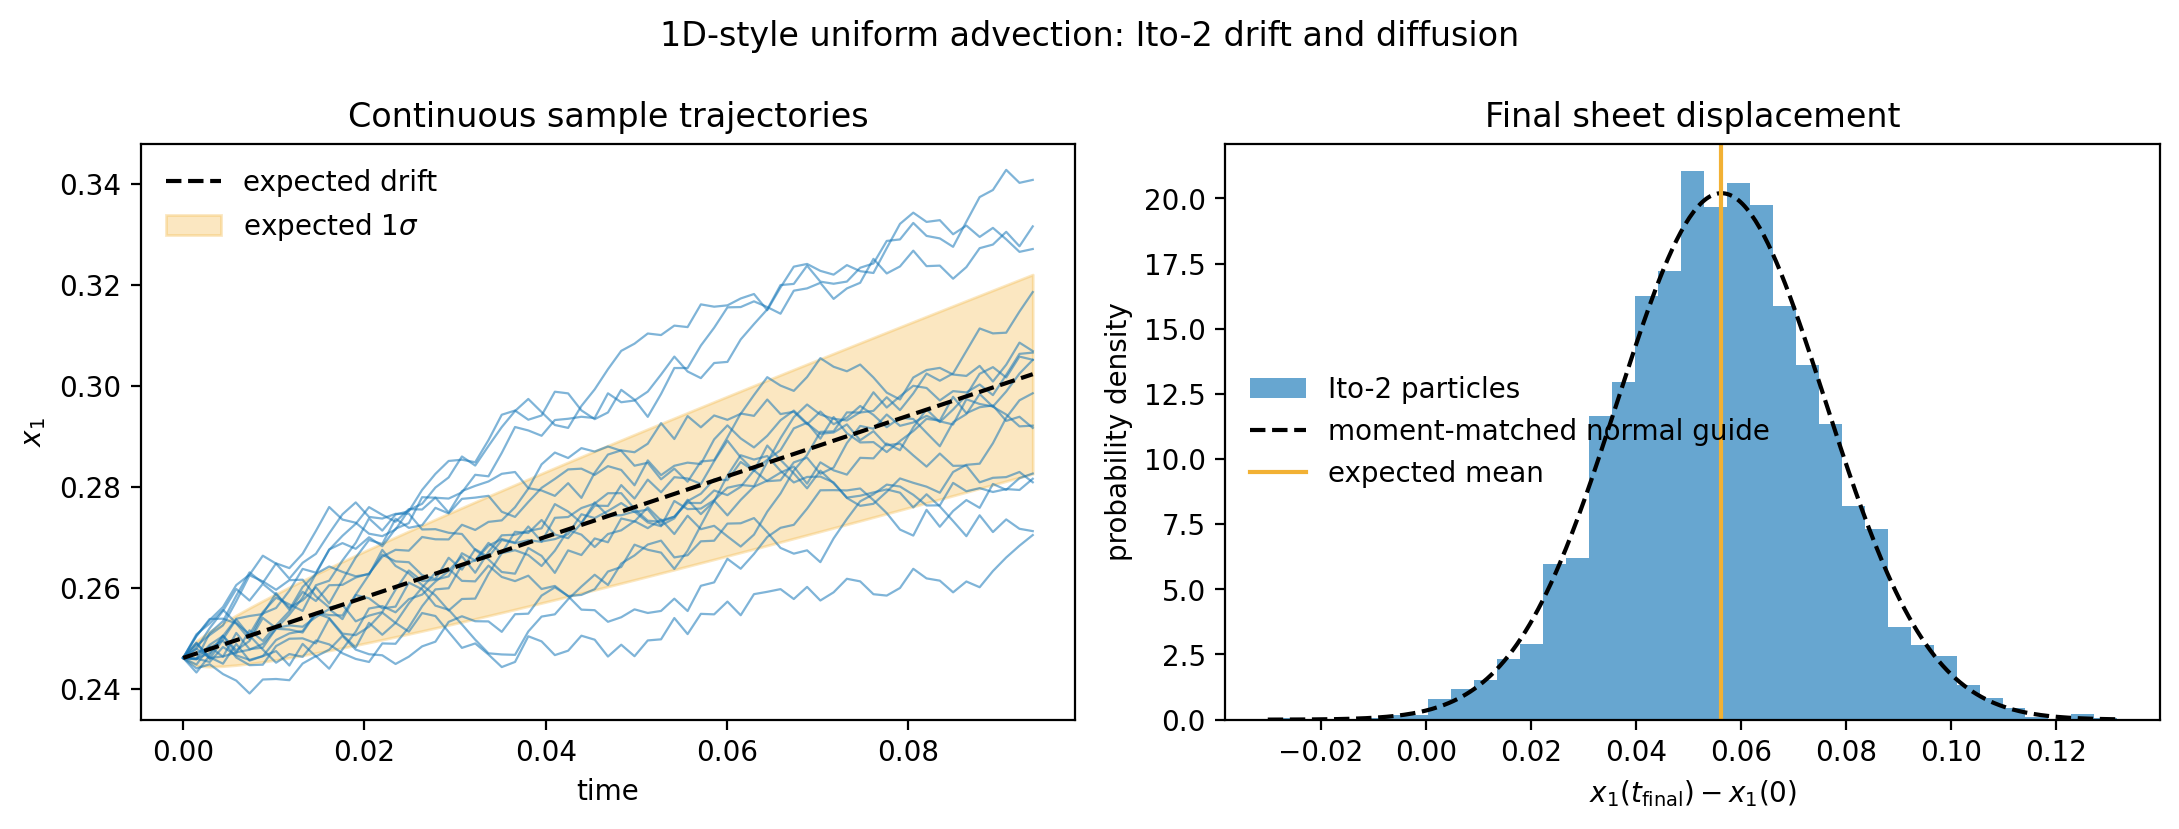
\includegraphics[width=\textwidth]{ito_tracers_1d_sheet.png}
\caption{Committed one-dimensional-style behavior test generated by
\texttt{plot\_ito\_tracer\_figures.py}. The paths are continuous, while
the final distribution follows the expected Monte Carlo mean and variance.
The measured final mean displacement is \(0.05616\), compared with the expected
\(0.05625\). This supports per-coordinate moment matching; it does not claim
that the continuous distribution reproduces every higher moment of the
discrete jump process.}
\label{fig:one-d}
\end{figure}

The CPU regression computes the expected mean
\(\langle\Delta x\rangle=v\Delta t\) and variance
\(h^2 C(1-C)\) for uniform advection, then checks 4096-particle samples against
those values. It also checks restart behavior and verifies that \Ito{}-3 and
invalid particle-type combinations are rejected.

\subsection{Two-dimensional continuous paths}

\begin{figure}[htbp]
\centering
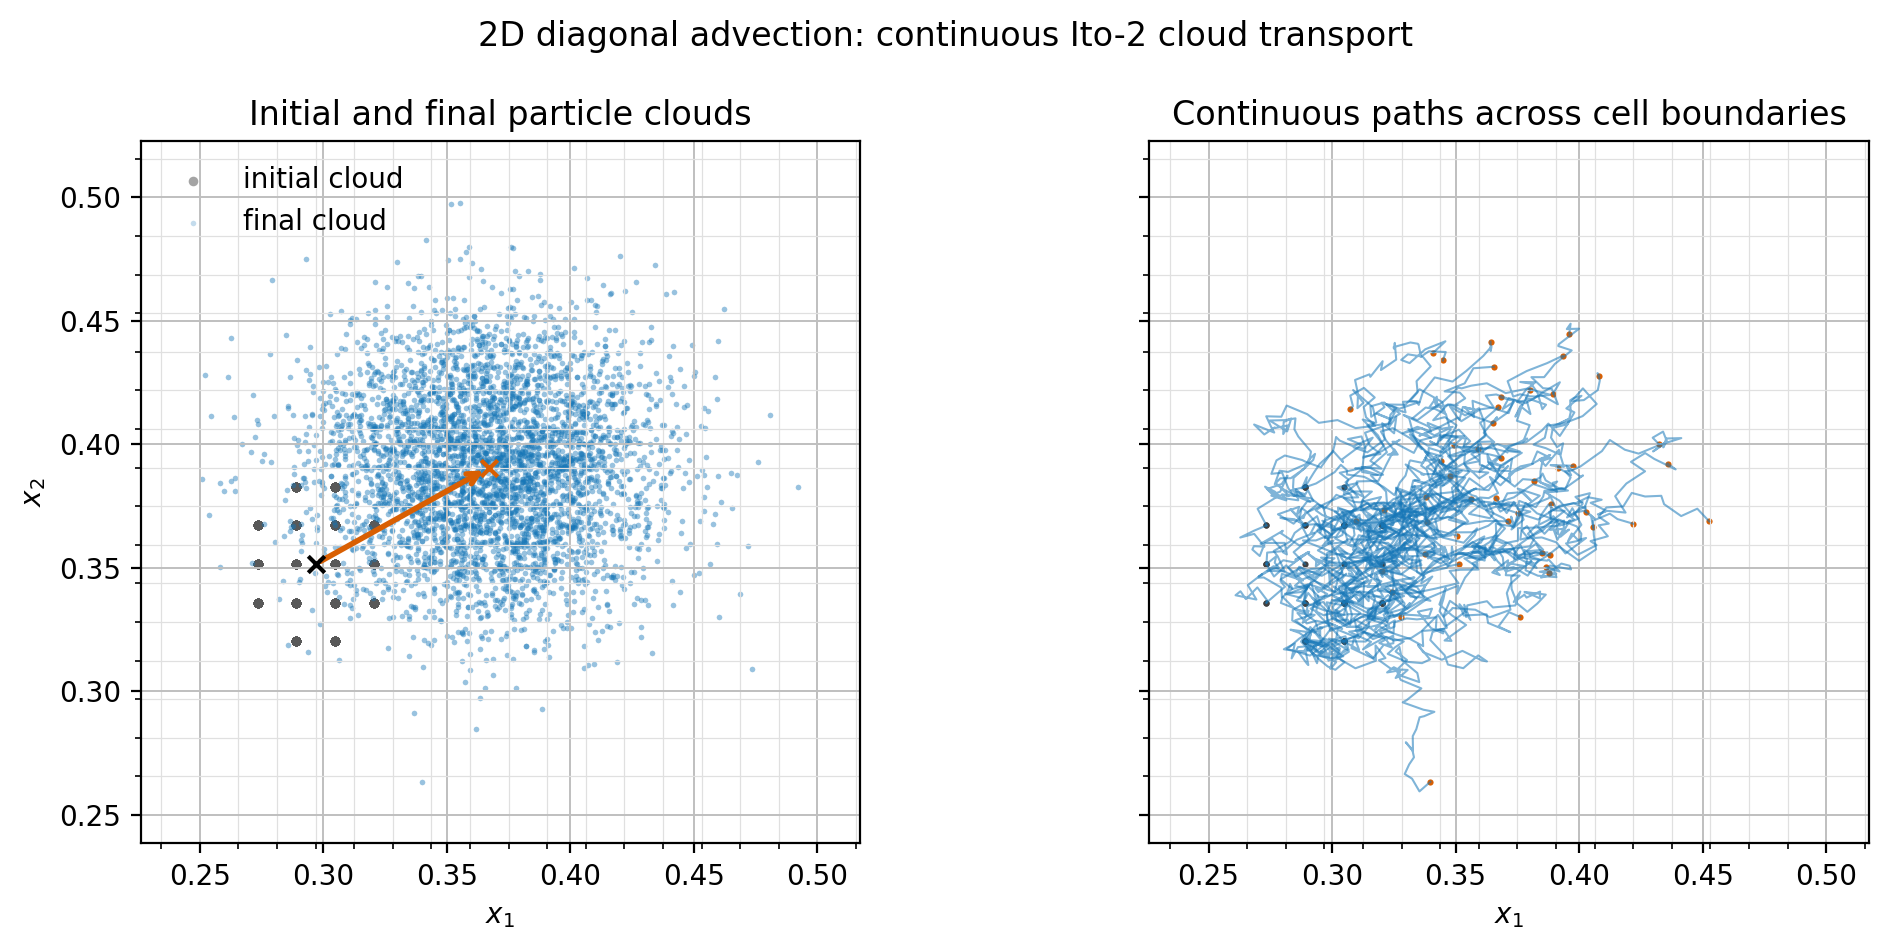
\includegraphics[width=0.96\textwidth]{ito_tracers_2d_cloud.png}
\caption{Committed two-dimensional cloud test generated by
\texttt{plot\_ito\_tracer\_figures.py}. The final cloud both advects and
spreads, and the sample paths remain continuous rather than snapping between
cell centers. This is direct evidence for the intended geometric behavior, but
it is not by itself a test of thermodynamic sampling or AMR communication.}
\label{fig:two-d}
\end{figure}

The two-dimensional cloud uses 4096 tracers on a \(64\times64\) mesh with
diagonal velocity \((v_1,v_2)=(0.45,0.25)\). Separate MPI/AMR regression
coverage checks that particles migrate across ranks, preserve continuous
subcell positions through refinement boundaries, and restart from per-rank
restart files.

\section{Thermodynamic Tracing of Thermal Instability}

\subsection{Physical setup}

The more informative integration experiment combines the \Ito{}-2 particles
with ISM-like cooling and initial perturbations in a periodic
\(20\,\mathrm{pc}\times20\,\mathrm{pc}\), \(128^2\) Hydro calculation. The gas
starts in exact heating-cooling balance at
\begin{equation}
  \frac{P}{k_B}=3000\ \mathrm{K\,cm^{-3}},
  \qquad
  n_0=1.9071755\ \mathrm{cm^{-3}},
  \qquad
  T_0=1573.0068\ \mathrm{K}.
\end{equation}
This is the unstable middle equilibrium. At the initial pressure, the stable
equilibria are near \(52\) K and \(6353\) K.

The causal chain is simple. The \(1\%\) density-only perturbations leave the
initial temperature uniform. Slightly denser regions cool faster because
radiative cooling scales as \(n^2\), while constant per-particle heating scales
as \(n\). They lose pressure and condense. Slightly underdense regions net heat
and expand. The 4096 mass-weighted \Ito{} tracers record which thermal phase
their stochastic mass-flux trajectories occupy over time.

\begin{landscape}
\begin{figure}[p]
\centering
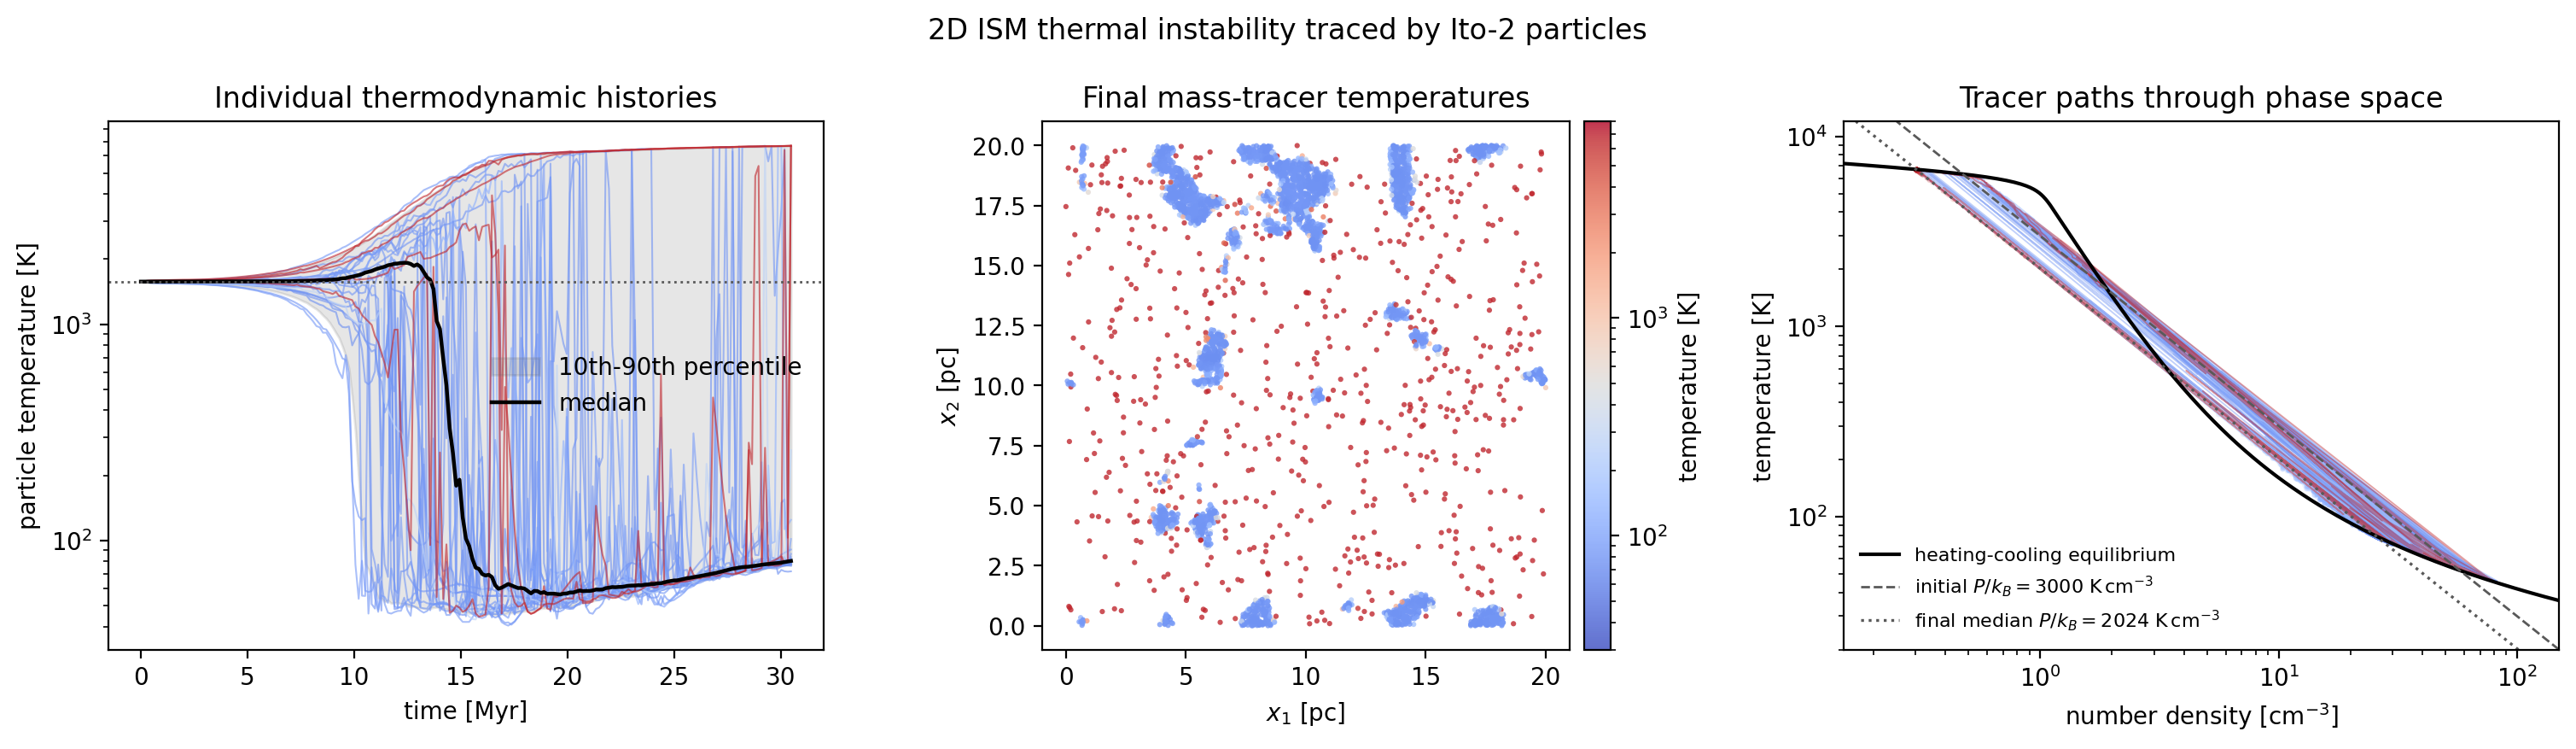
\includegraphics[width=0.98\linewidth]{ito_tracers_thermal_instability_2d.png}
\caption{Thermodynamic tracing in the two-dimensional thermal-instability
experiment, generated by \texttt{plot\_ito\_thermal\_instability.py}.
Look first at the left panel: the initially single-temperature population
separates into cold and warm histories. The middle panel shows the final
mass-tracer temperatures. In the right panel, paths approach the two stable
intersections of the heating-cooling equilibrium curve with the evolved median
isobar. Sharp jumps in individual histories occur when a particle crosses a
thin phase interface because history output samples the fluid cell containing
the particle. The figure supports coupled thermodynamic tracing; it does not
establish resolution-converged interface structure or fragmentation.}
\label{fig:thermal}
\end{figure}
\end{landscape}

\subsection{Observed result}

The run completed 100 code time units, or \(30.47\) Myr, in 9437 cycles. Its
thermodynamic-history output contained 823,296 finite records over 201 output
cycles for all 4096 tags. At the final output:

\begin{itemize}
  \item the mass-weighted median pressure was
        \(P/k_B=2024\ \mathrm{K\,cm^{-3}}\);
  \item the cooling curve's stable roots at that pressure were \(79.5\) K and
        \(6720\) K, separated by an unstable root at \(589\) K;
  \item the measured median tracer temperatures were \(79.5\) K in the cold
        phase and \(6673\) K in the warm phase; and
  \item the mass-tracer fractions were \(81.8\%\) below \(300\) K,
        \(15.5\%\) above \(5000\) K, and \(2.7\%\) between those thresholds.
\end{itemize}

The agreement between the measured phase temperatures and the stable
heating-cooling intersections is the strongest evidence that the particles are
recording the expected thermodynamic evolution. Because the particles were
seeded by mass, the reported fractions estimate mass fractions, not volume
fractions.

\section{Verification and Failure Boundaries}

\begin{table}[htbp]
\centering
\small
\begin{tabularx}{\textwidth}{@{}p{0.25\textwidth}X p{0.20\textwidth}@{}}
\toprule
Check & Evidence & Status \\
\midrule
Uniform-flow moments
& CPU regression compares 4096-particle mean and variance with the analytical
  Monte Carlo moments; includes RK2 and RK3.
& \status{Passed} \\
\addlinespace
Restart and invalid requests
& Serial restart passes; \Ito{}-3, order 3, and wrong particle-type
  combinations are explicitly rejected.
& \status{Passed} \\
\addlinespace
MHD, MPI, and AMR
& Core \Ito{} validation includes MHD thermodynamic fields and a two-rank
  MPI/AMR migration and restart regression that checks continuous subcell
  positions.
& \status{Passed for core implementation} \\
\addlinespace
Merged cooling and perturbation integration
& Combined serial build and 43 focused \Ito{}, cooling, and initial-perturbation
  tests.
& \status{Passed} \\
\addlinespace
Thermal-instability experiment
& Full \(128^2\), 4096-particle run completed with all history values finite and
  phase temperatures consistent with stable equilibria.
& \status{Passed} \\
\addlinespace
Merged-feature MPI integration
& No additional MPI run was performed after merging cooling and initial
  perturbations into the \Ito{} branch.
& \status{Not tested} \\
\bottomrule
\end{tabularx}
\caption{Verification status. The distinction between core \Ito{} MPI
validation and the later merged-feature serial validation is intentional.}
\end{table}

The fail-closed checks are part of the implementation, not just the tests.
Runs terminate on invalid or non-finite Monte Carlo probabilities, negative
diffusion beyond tolerance, invalid interpolated coefficients, non-finite
displacements, and displacements that would cross more than one MeshBlock in
an active direction.

\section{What the Work Supports, and What It Does Not}

\textbf{What is directly supported.}
\begin{itemize}
  \item \Ito{}-2 is integrated with the existing Monte Carlo mass-tracer
        infrastructure and final finite-volume mass fluxes.
  \item Controlled tests support the intended per-coordinate first- and
        second-moment matching and continuous-path behavior.
  \item The particles can record interpretable mass-weighted thermodynamic
        histories in a coupled two-phase cooling calculation.
\end{itemize}

\textbf{What remains uncertain or explicitly unsupported.}
\begin{itemize}
  \item No \Ito{}-3 or third-moment method is implemented or validated.
  \item Independent coordinate kicks do not claim to reproduce the full joint
        discrete jump distribution or all higher moments.
  \item Current support is limited to non-relativistic Cartesian Hydro/MHD,
        periodic active boundaries, dynamic RK1--RK3 evolution, and 2D/3D
        particle meshes.
  \item The existing particle migration path limits a realized displacement to
        less than one MeshBlock per coordinate per fluid timestep.
  \item The thermal-instability experiment omits conduction, so the Field
        length is unresolved. Interface thickness, small condensations, and
        phase fractions are resolution-, seed-, domain-, and runtime-dependent.
  \item The final particle map samples the mass distribution; it is not a
        complete volume-filling gas-temperature map.
\end{itemize}

\textbf{Bottom line.} \AthenaK{} now has a deliberately scoped \Ito{}-2
mass-flux tracer that converts the existing Monte Carlo jump statistics into
continuous stochastic paths without disconnecting the particles from the
finite-volume mass transport. The thermodynamic-tracing use case works, while
third-order behavior, unrestricted configurations, full joint-distribution
matching, and converged thermal fragmentation remain outside the supported
claim.

\section{Reproduction and Artifact Map}

The thermal-instability experiment and figure can be reproduced from the
repository root with:

\begin{verbatim}
./build/src/athena \
  -i inputs/particles/ito_tracers_thermal_instability_2d.athinput \
  -d run_ito_ti_2d

python scripts/plot_ito_thermal_instability.py \
  run_ito_ti_2d/prtcl_thermo_history/\
ito_tracers_thermal_instability_2d.prtcl_thermo_history.thp
\end{verbatim}

\textbf{Implementation:}
\texttt{particles\_lagrangian\_ito.cpp}, \texttt{driver.cpp}, the Hydro/MHD
flux files, and \texttt{particles\_tasks.cpp}.

\textbf{Regression evidence:}
\texttt{test\_particles\_ito\_cpu.py} and
\texttt{test\_particles\_ito\_mpicpu.py}.

\textbf{Thermal experiment:}
\artifact{inputs/particles/ito_tracers_thermal_instability_2d.athinput}.
Figure script: \artifact{scripts/plot_ito_thermal_instability.py}.

\textbf{User documentation:} \texttt{docs/source/modules/ito\_tracers.md}.

\end{document}
